\section{Trabalhos Relacionados}

Durante a pesquisa bibliográfica realizada neste trabalho, encontrou-se alguns trabalhos que também fizeram análise de textos parlamentares utilizando aprendizado Bayesiano. As seções a seguir descrevem brevemente alguns deles.

\subsection{Retórica Parlamentar}

O Retórica Parlamentar\footnote{http://retorica.labhackercd.net/about.html}, idealizado por Davi Moreira\footnote{https://github.com/davi-moreira}, Manoel Galdino\footnote{https://github.com/mgaldino} e Luís Carli\footnote{https://github.com/luiscarli}, utiliza os discursos proferidos pelos parlamentares no Pequeno Expediente e no Grande Expediente da Câmara dos Deputados para promover a transparência do mandato e fornecer subsídios para o controle social com a divulgação dos temas mais debatidos em Plenário.

A técnica utilizada pelo Retórica para a classificação dos discursos é um modelo Bayesiano hierárquico, descrito por \citeonline{grimmer2009}, onde através de aprendizado não supervisionado são gerados \(k\) \textit{clusters}, sendo \(k\) um valor escolhido ao executar o algoritmo. O resultado é exportado para o formato \textit{csv} e contém os termos mais frequentes de cada cluster. Em seguida, um especialista deve ler e rotular cada \textit{cluster}.

A visualização dos dados é feita através de um gráfico de bolhas, em que cada bolha representa a relevância (medida pela frequência) de cada tema dentre todos os deputados analisados. Dentro de cada bolha são colocados os deputados que enfatizam aquele tema nos seus discursos. Um deputado está associado a um único tema, que é o tema mais enfatizado por ele nos seus discursos.

\begin{figure}[h]
    \centering
    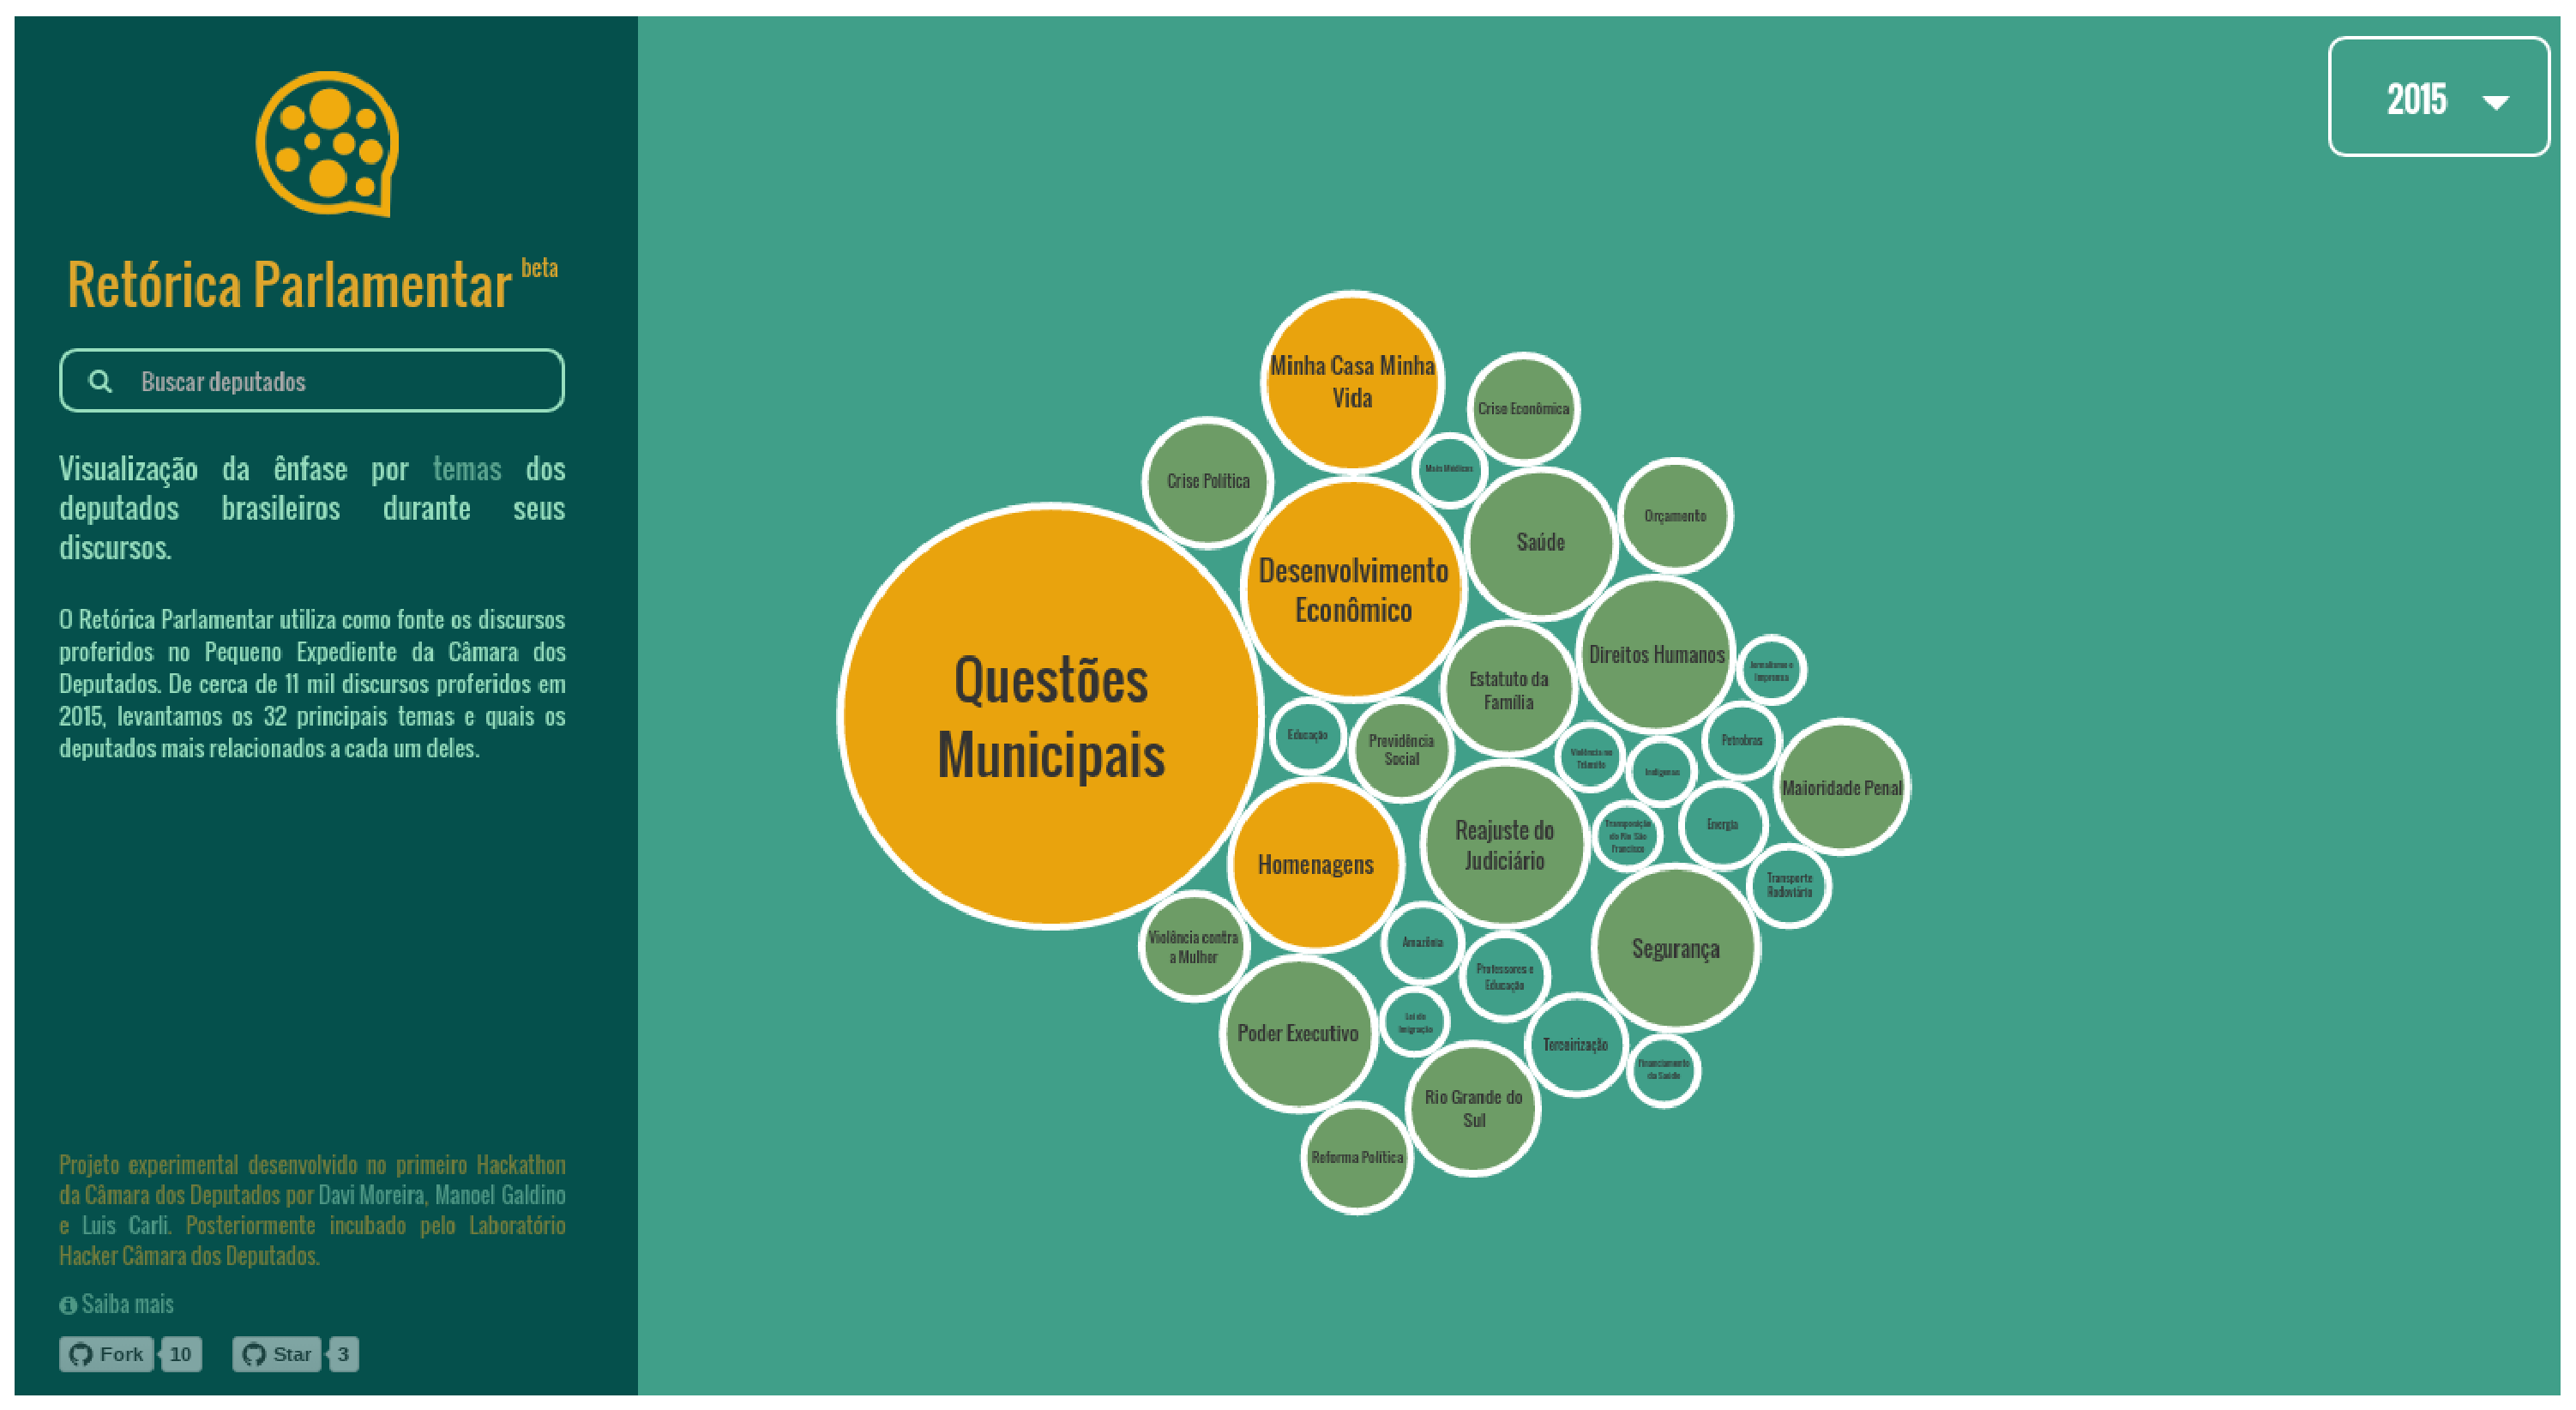
\includegraphics[scale=0.3]{figuras/retorica.eps}
    \caption{Retórica Parlamentar}
\end{figure}


\subsection{\textit{Automatic content analysis of legislative documents by text mining techniques}}

Outro trabalho encontrado foi o de \citeonline{lin}, onde propõem uma análise automática dos dados do parlamento de Taiwan, como questionamentos legislativos, discursos em conferências, proposições legislativas e proposições provisórias do Legislativo de Yuan (poder legislativo unicameral da República da China), utilizando técnicas de processamento de linguagem natural, com o objetivo de representar o desempenho de cada legislador em determinadas categorias, definidas por especialistas do \textit{Institute of Political Science} da \textit{National Sun Yat-sen University}.

\citeonline{lin} definem três aspectos para a análise dos dados do parlamento de Taiwan: direção geográfica, público-alvo e tópico. A direção geográfica se refere ao escopo geográfico abrangido pelos registros legislativos e tem 5 direções. O público-alvo refere-se às pessoas mencionadas explicitamente em seus registros, podendo ser 30 opções. O tópico inclui os temas abordados pelos parlamentares, que possuem um total de 29 tópicos. A figura abaixo mostra os três aspectos e seus valores correspondentes:

\clearpage

\begin{figure}[h]
    \centering
    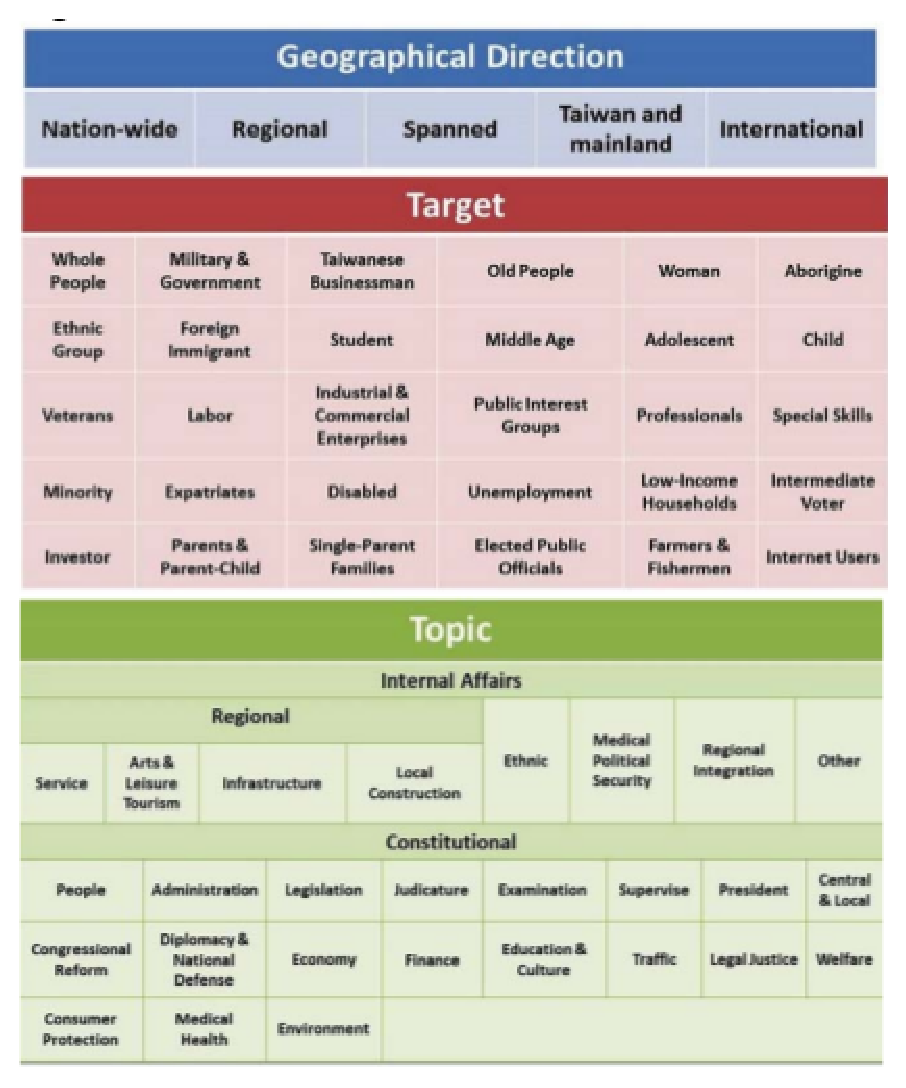
\includegraphics[scale=0.5]{figuras/aspects.eps}
    \caption{Estrutura de categorização}
\end{figure}


Após o processo de pré-processamento do texto, os dados passam por duas fases de clusterização. A primeira fase consiste em uma classificação hierárquica, com o objetivo de obter o número de \textit{clusters} ideal. Em seguida, é aplicado o \textit{k-means}, utilizando o número obtido no processo anterior como valor de \(k\). Dessa forma conseguem melhorar a relevância dos termos que serão apresentados aos especialistas para a definição dos termos que representam as classes.

Os autores disponibilizaram uma interface \textit{web} para os especialistas, para que eles classificassem os quatro tipos de texto (questionamentos legislativos, discursos em conferências, proposições legislativas e proposições provisórias). Esses textos classificados serviram como dados de treinamento e teste do modelo \textit{Support Vector Machine}, adotado para fazer a classificação.

Para representar os dados da análise, foram utilizados gráficos de radar para cada aspecto mencionado anteriormente, como mostram as figuras:

\begin{figure}[h]
  \centering
  \begin{subfigure}{.3\textwidth}
    \centering
    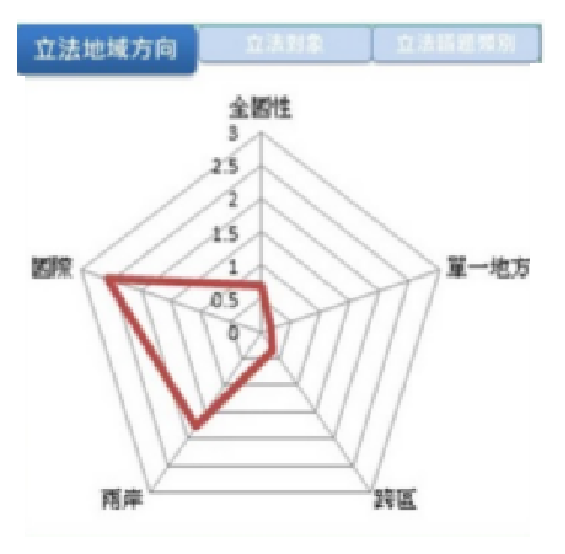
\includegraphics[scale=0.35]{figuras/aspecto1.eps}
  \end{subfigure}%
  \begin{subfigure}{.3\textwidth}
    \centering
    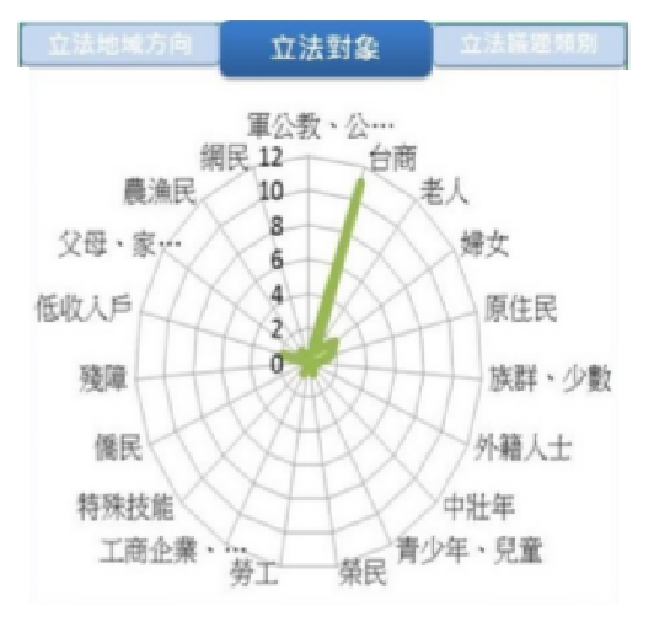
\includegraphics[scale=0.3]{figuras/aspecto2.eps}
  \end{subfigure}
  \begin{subfigure}{.3\textwidth}
    \centering
    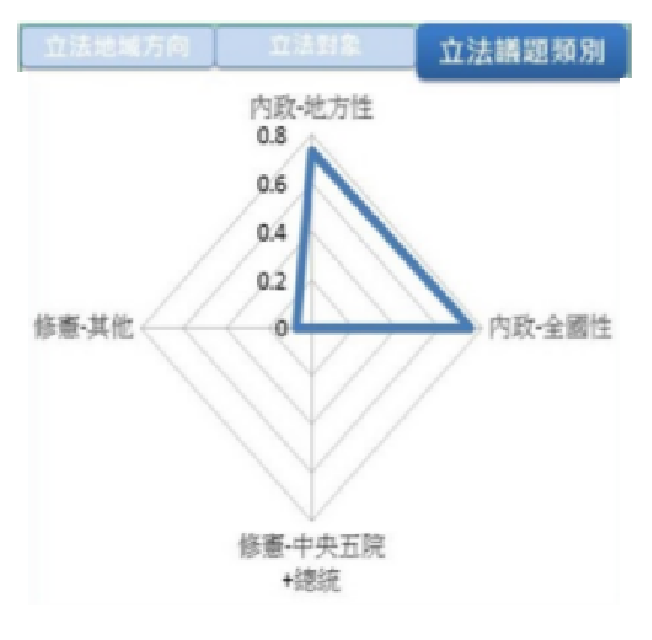
\includegraphics[scale=0.3]{figuras/aspecto3.eps}
  \end{subfigure}
  \caption{Gráficos de desempenho do parlamentar}
\end{figure}
